\section{Линейные фильтры}

Для выполнения задания рассмотрим функцию $g(t)$, которая задается следующим образом: 
\begin{equation}
    g(t) = \begin{cases}
        a, & t \in [t_1, t_2]\\
        0, & otherwise
    \end{cases}
\end{equation}

Кроме того, зададим \textit{зашумленную} версию функции $u(t)$ 
\begin{equation}
    u(t) = g(t) + b(\rand(t) - 0.5) + c(\sin(d \cdot t))  
    \label{eq:noise}
\end{equation}


\subsection{Линейный фильтр первого порядка}

Будем рассматривать линейный фильтр первого порядка, который описывается следующим уравнением:
\begin{equation}
    W_1(p) = \frac{1}{Tp + 1}
\end{equation}
где $T$ -- постоянная времени.

\def\num{1}
\def\a{4}
\def\from{1}
\def\to{4}
\def\b{1}
\def\c{0}
\def\d{0}
\def\L{10}
\def\T{0.5}

\subsubsection{Рассматриваемая функция}
Рассмотрим функцию $g(t)$ при параметрах $a=\a$, $t_1 = \from$, $t_2 = \to$ ~(см. рисунок~\ref{fig:wave_func_\num}) 
и ее \textit{зашумленную} версию $u(t)$ с параметрами $b = \b$, $c = \c$, $d = \d$ ~(см. рисунок~\ref{fig:noised_wave_func_\num}).
на промежутке $[0,\L]$. 

\subsubsection{Графики рассматриваемой и зашумленной функции}
\begin{figure}[ht!]
    \centering
    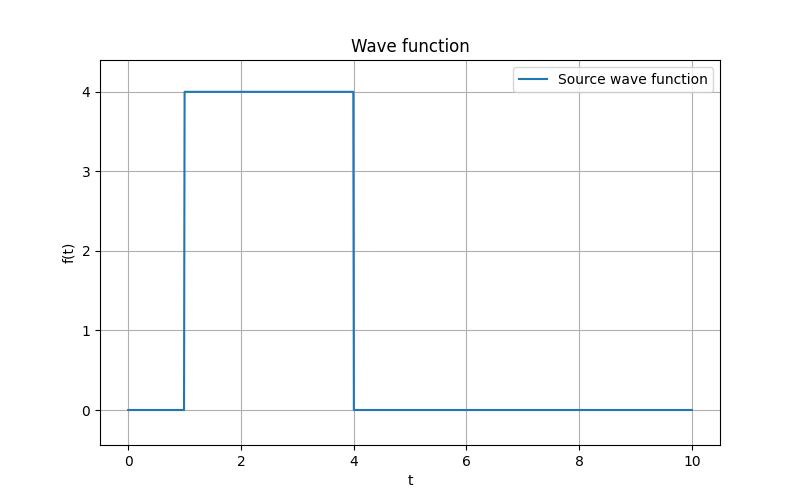
\includegraphics[width=\textwidth]{../results/second/\num/wave_func.png}
    \caption{Функция $g(t)$ с параметрами $a = \a$, $t_1 = \from$, $t_2 = \to$}
    \label{fig:wave_func_\num}
\end{figure}

\begin{figure}[ht!]
    \centering
    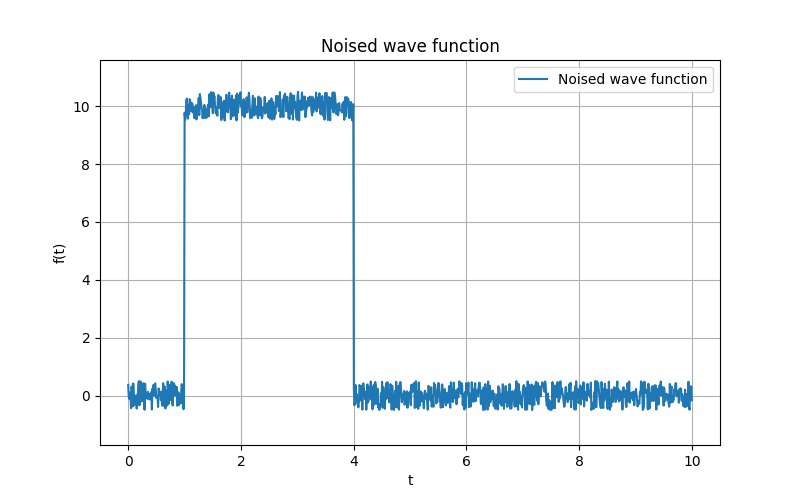
\includegraphics[width=\textwidth]{../results/second/\num/noised_wave_func.png}
    \caption{Функция $u(t)$ с параметрами $b = \b$, $c = \c$, $d = \d$}
    \label{fig:noised_wave_func_\num}
\end{figure}

\FloatBarrier
\subsubsection{Применение фильтра}

Рассмотрим фильтрованную функцию $u'(t)$, которая получается применением линейного фильтра первого порядка с $T = \T$ (см. рисунок \ref{fig:noised_wave_func_filtered_\num}).

\begin{figure}[ht!]
    \centering
    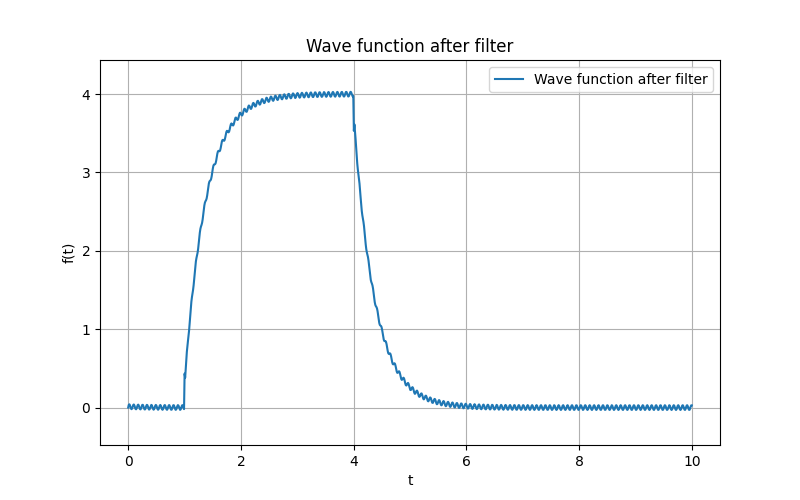
\includegraphics[width=\textwidth]{../results/second/\num/noised_wave_func_filtered.png}
    \caption{Функция $u'(t)$ после применения фильтра}
    \label{fig:noised_wave_func_filtered_\num}
\end{figure}

Видим, что функция после фильтрации стала более гладкой, фронт и спад стали менее выраженными. 
Это связано с тем, что фильтр убирает высокочастотные компоненты функции. Убедиться в этом можно 
рассмотрев АЧХ данного фильтра (см. рисунок \ref{fig:filter_frequency_response_\num}).

\FloatBarrier
\subsubsection{Аплитудно-частотная характеристика фильтра}
\begin{figure}[ht!]
    \centering
    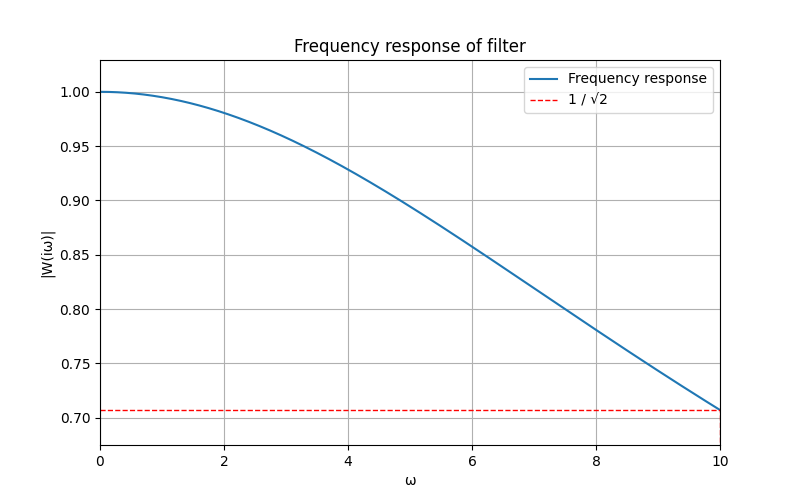
\includegraphics[width=\textwidth]{../results/second/\num/filter_frequency_response.png}
    \caption{АЧХ фильтра первого порядка при $T = \T$}
    \label{fig:filter_frequency_response_\num}
\end{figure}

На графике также отмечено значение $\omega_c$ -- \textit{частоты среза} $|W(i\omega_c)| = \frac{1}{\sqrt{2}}$, по нему можно судить о том, какие частоты будут \textit{усиливаться}, а какие \textit{подавляться}. 
Для фильтра первого порядка это значение равно $\omega_c = \frac{1}{T}$. Таким образом, делаем вывод, что все частоты, 
большие $\frac{1}{\T} = \fpeval{1/ \T}$ будут подавляться, что соответствует значению на графике. 

\FloatBarrier
\subsubsection{Результаы фильтрации}
Сравнительный график исходной функции и функции после фильтрации представлен на рисунке \ref{fig:wave_func_cmp_\num}.

\begin{figure}[ht!]
    \centering
    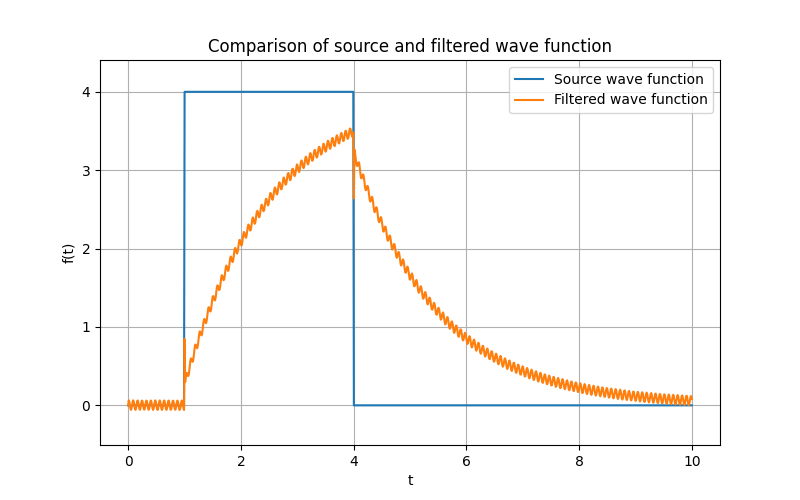
\includegraphics[width=\textwidth]{../results/second/\num/wave_func_cmp.png}
    \caption{Сравнение функции $g(t)$ и $u'(t)$}
    \label{fig:wave_func_cmp_\num}
\end{figure}

Образ исходной функции и функции после фильтрации приведены на рисунках \ref{fig:wave_func_image_\num}~и~\ref{fig:noised_wave_func_filtered_image_\num}.
Графики модулей соответствующих функций приведены на рисунках~\ref{fig:wave_func_image_abs_\num}~и~\ref{fig:noised_wave_func_filtered_image_abs_\num}, их 
сравнительный график -- на рисунке~\ref{fig:wave_func_image_cmp_\num}.

\begin{figure}[ht!]
    \centering
    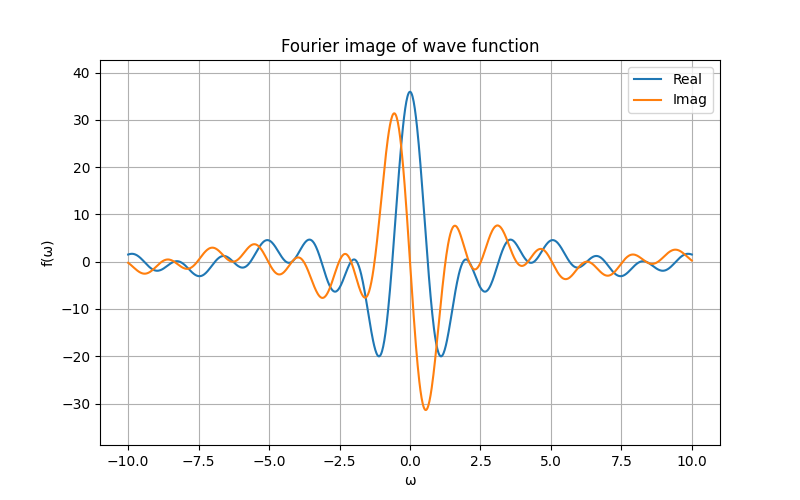
\includegraphics[width=\textwidth]{../results/second/\num/wave_func_image.png}
    \caption{Образ исходной функции $u(t)$.}
    \label{fig:wave_func_image_\num}
\end{figure}

\begin{figure}[ht!]
    \centering
    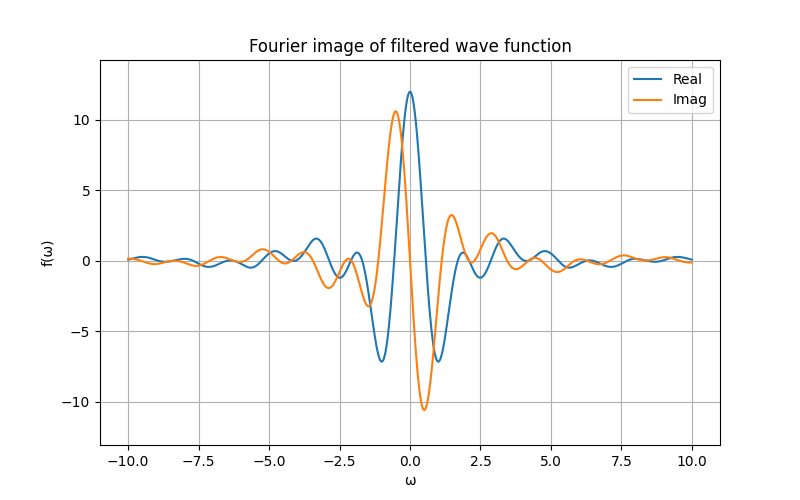
\includegraphics[width=\textwidth]{../results/second/\num/noised_wave_func_filtered_image.png}
    \caption{Образ фильтрованной функции $u'(t)$.}
    \label{fig:noised_wave_func_filtered_image_\num}
\end{figure}

\begin{figure}[ht!]
    \centering
    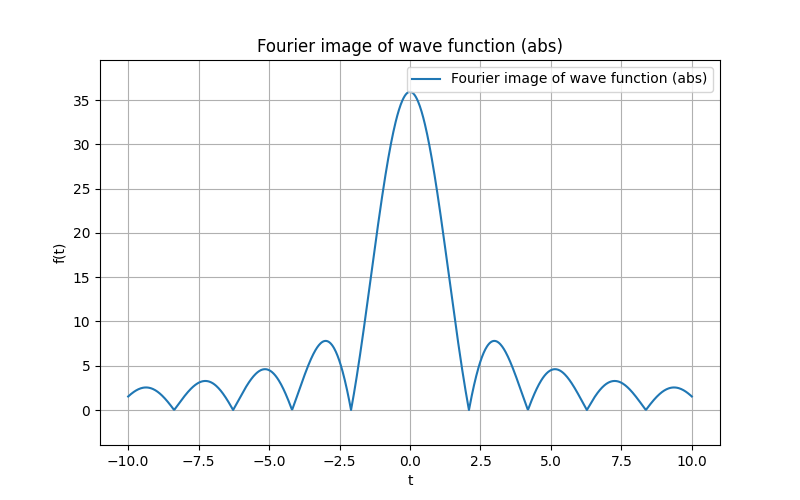
\includegraphics[width=\textwidth]{../results/second/\num/wave_func_image_abs.png}
    \caption{Модуль образа исходной функции $u(t)$.}
    \label{fig:wave_func_image_abs_\num}
\end{figure}

\begin{figure}[ht!]
    \centering
    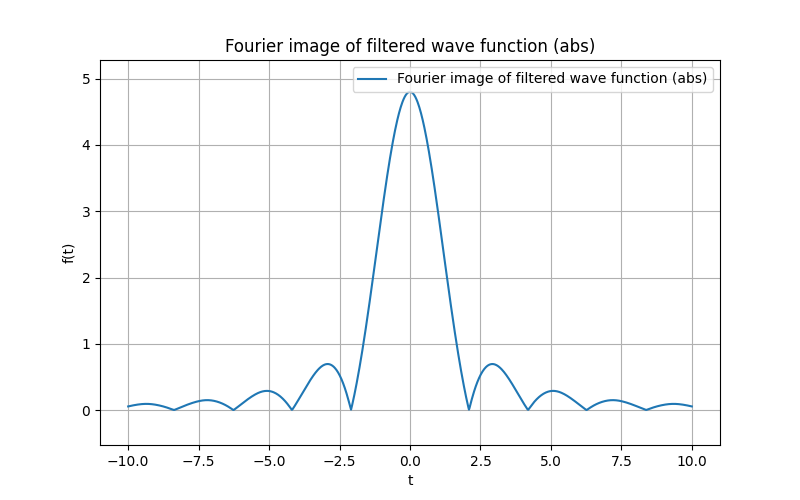
\includegraphics[width=\textwidth]{../results/second/\num/noised_wave_func_filtered_image_abs.png}
    \caption{Модуль образа фильтрованной функции $u'(t)$.}
    \label{fig:noised_wave_func_filtered_image_abs_\num}
\end{figure}

\begin{figure}[ht!]
    \centering
    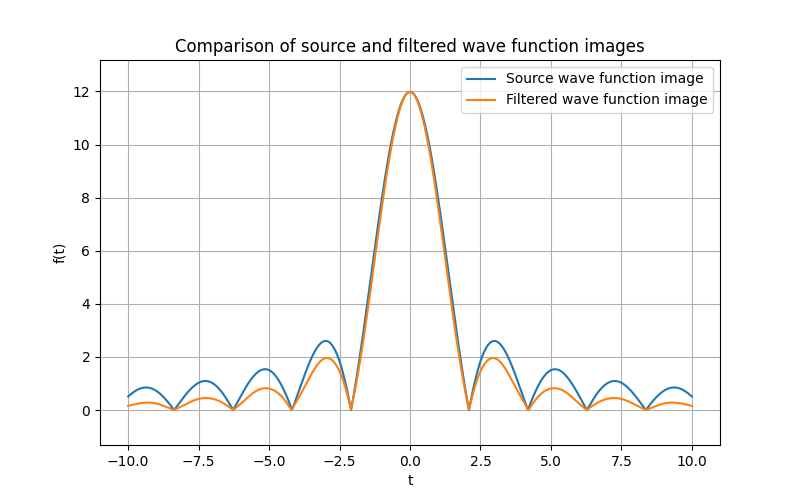
\includegraphics[width=\textwidth]{../results/second/\num/wave_func_image_cmp.png}
    \caption{Сравнение модулей образов исходной и фильтрованной функций.}
    \label{fig:wave_func_image_cmp_\num}
\end{figure}

На графиках модуля исходного и фильтрованного сигнала видно, что фильтр убирает высокочастотные компоненты, что и приводит к сглаживанию функции.

\FloatBarrier
\def\num{2}
\def\T{0.3}
Рассмотрим линейный фильтр первого порядка при $T = \T$ (см. рисунок \ref{fig:noised_wave_func_filtered_\num}).

\begin{figure}[ht!]
    \centering
    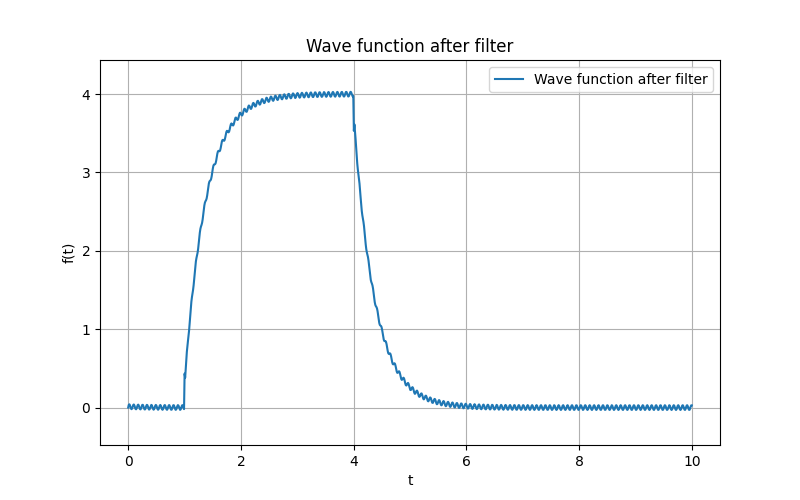
\includegraphics[width=\textwidth]{../results/second/\num/noised_wave_func_filtered.png}
    \caption{Функция $u'(t)$ после применения фильтра}
    \label{fig:noised_wave_func_filtered_\num}
\end{figure}
В данном случае фронт и спад стали более резкими, функция стала больше похожа на исходную. 
АЧХ данного фильтра представлена на рисунке \ref{fig:filter_frequency_response_\num}.

\begin{figure}[ht!]
    \centering
    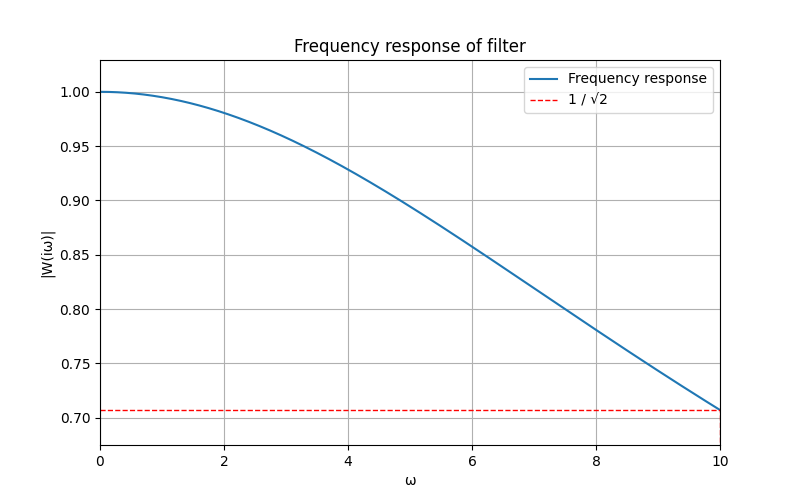
\includegraphics[width=\textwidth]{../results/second/\num/filter_frequency_response.png}
    \caption{АЧХ фильтра первого порядка при $T = \T$}
    \label{fig:filter_frequency_response_\num}
\end{figure}
В данном случае будут подавляться частоты большие $\frac{1}{\T} = \fpeval{round(1/ \T, 3)}$, что значит, что функция лучше повторяет исходную,
по сравнению с прошлой. 

Сравнительный график исходной функции и функции после фильтрации представлен на рисунке \ref{fig:wave_func_cmp_\num}.

Образ исходной функции и функции после фильтрации приведены на рисунках \ref{fig:wave_func_image_\num}~и~\ref{fig:noised_wave_func_filtered_image_\num}.
Графики модулей соответствующих функций приведены на рисунках~\ref{fig:wave_func_image_abs_\num}~и~\ref{fig:noised_wave_func_filtered_image_abs_\num}, их 
сравнительный график -- на рисунке~\ref{fig:wave_func_image_cmp_\num}.

\begin{figure}[ht!]
    \centering
    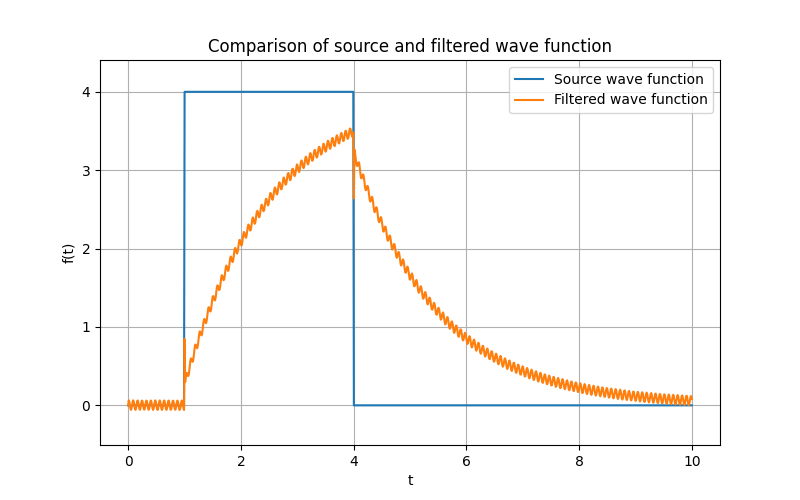
\includegraphics[width=\textwidth]{../results/second/\num/wave_func_cmp.png}
    \caption{Сравнение функции $g(t)$ и $u'(t)$}
    \label{fig:wave_func_cmp_\num}
\end{figure}

\begin{figure}[ht!]
    \centering
    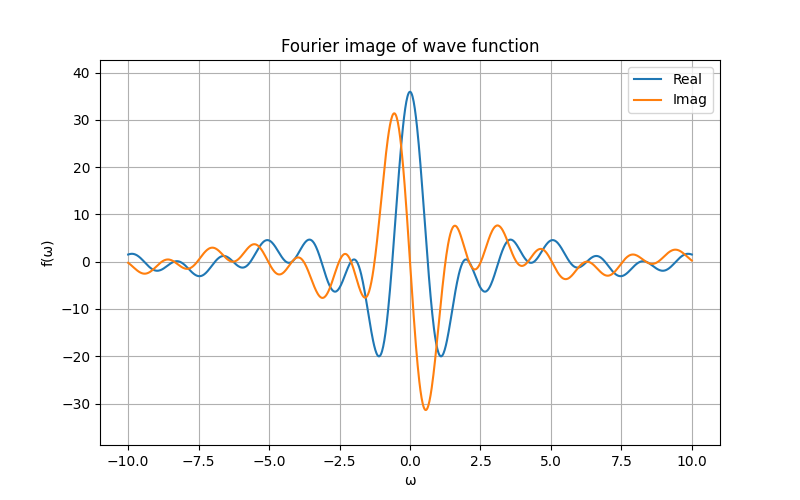
\includegraphics[width=\textwidth]{../results/second/\num/wave_func_image.png}
    \caption{Образ исходной функции $u(t)$.}
    \label{fig:wave_func_image_\num}
\end{figure}

\begin{figure}[ht!]
    \centering
    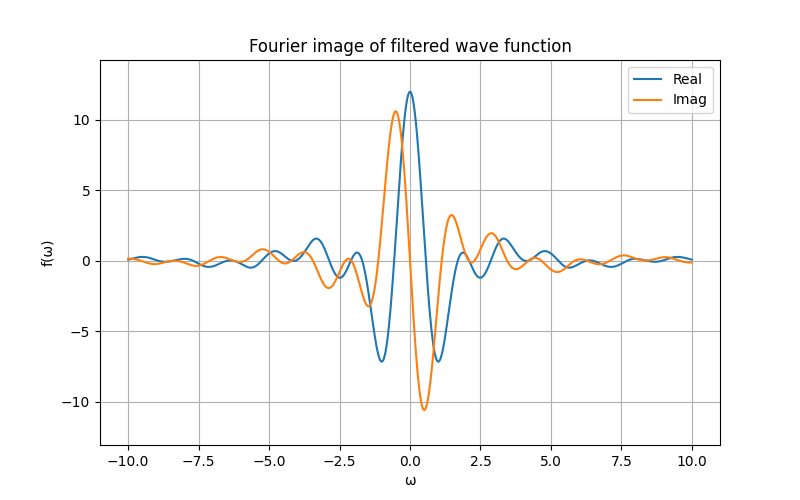
\includegraphics[width=\textwidth]{../results/second/\num/noised_wave_func_filtered_image.png}
    \caption{Образ фильтрованной функции $u'(t)$.}
    \label{fig:noised_wave_func_filtered_image_\num}
\end{figure}

\begin{figure}[ht!]
    \centering
    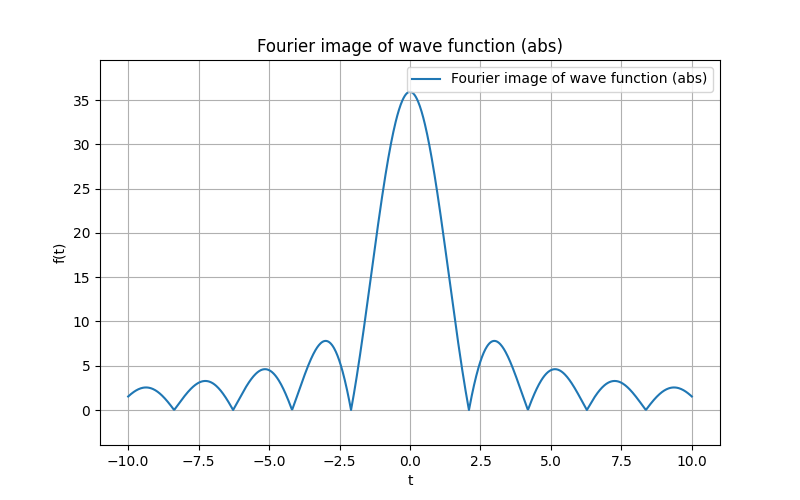
\includegraphics[width=\textwidth]{../results/second/\num/wave_func_image_abs.png}
    \caption{Модуль образа исходной функции $u(t)$.}
    \label{fig:wave_func_image_abs_\num}
\end{figure}

\begin{figure}[ht!]
    \centering
    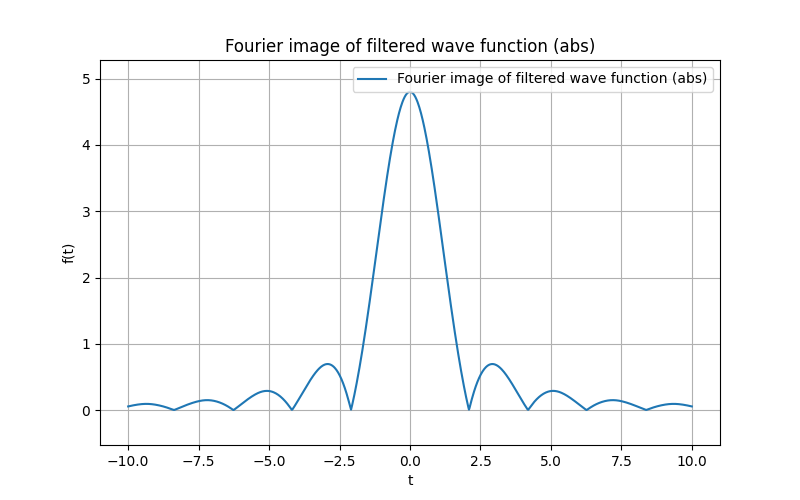
\includegraphics[width=\textwidth]{../results/second/\num/noised_wave_func_filtered_image_abs.png}
    \caption{Модуль образа фильтрованной функции $u'(t)$.}
    \label{fig:noised_wave_func_filtered_image_abs_\num}
\end{figure}

\begin{figure}[ht!]
    \centering
    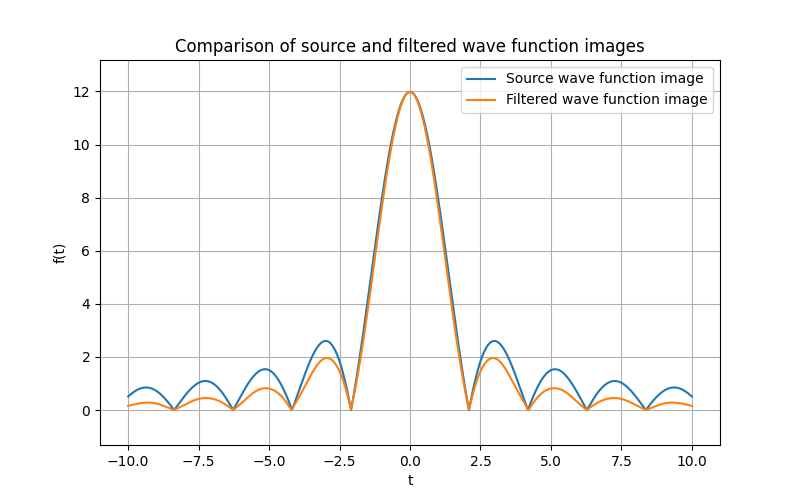
\includegraphics[width=\textwidth]{../results/second/\num/wave_func_image_cmp.png}
    \caption{Сравнение модулей образов исходной и фильтрованной функций.}
    \label{fig:wave_func_image_cmp_\num}
\end{figure}


\FloatBarrier
\def\num{3}
\def\T{0.1}
Также посмотрим на фильтр с параметром $T = \T$ (см. рисунок \ref{fig:noised_wave_func_filtered_\num}).
\begin{figure}[ht!]
    \centering
    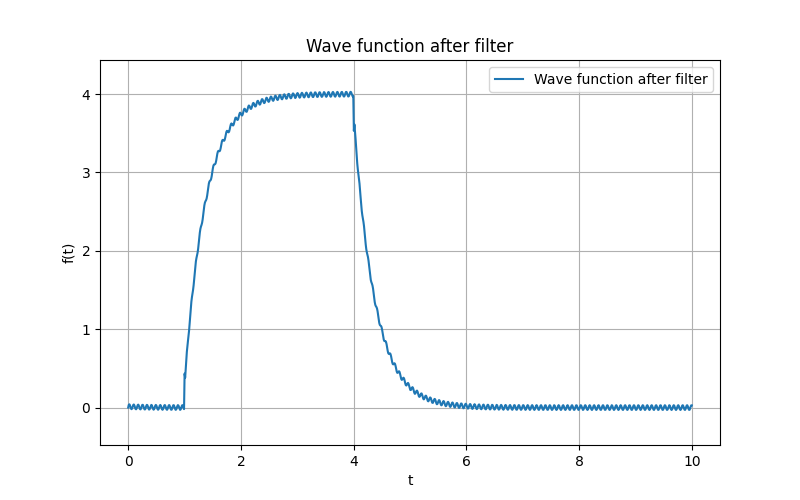
\includegraphics[width=\textwidth]{../results/second/\num/noised_wave_func_filtered.png}
    \caption{Функция $u'(t)$ после применения фильтра}
    \label{fig:noised_wave_func_filtered_\num}
\end{figure}
Теперь функция стала еще более похожей на исходную квадратную волну, но в фильтрованной функции 
стали проявляться шумы из исходной функции. 
АЧХ данного фильтра представлена на рисунке \ref{fig:filter_frequency_response_\num}.

\begin{figure}[ht!]
    \centering
    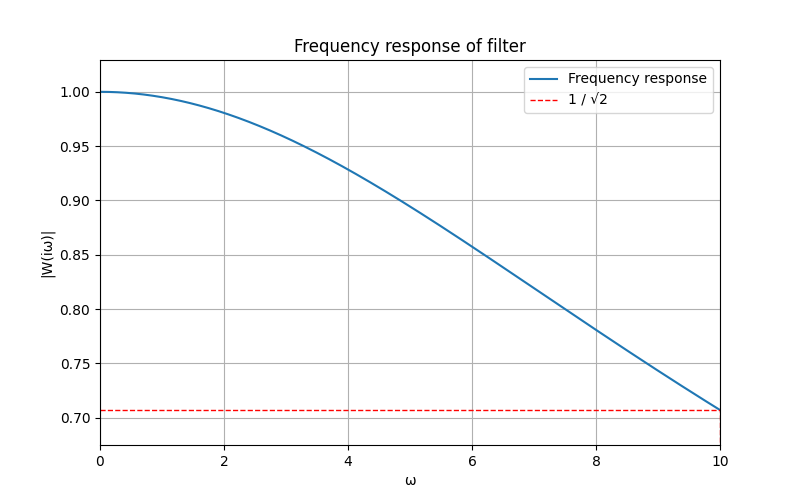
\includegraphics[width=\textwidth]{../results/second/\num/filter_frequency_response.png}
    \caption{АЧХ фильтра первого порядка при $T = \T$}
    \label{fig:filter_frequency_response_\num}
\end{figure}

Сравнительный график исходной функции и функции после фильтрации представлен на рисунке \ref{fig:wave_func_cmp_\num}.

\begin{figure}[ht!]
    \centering
    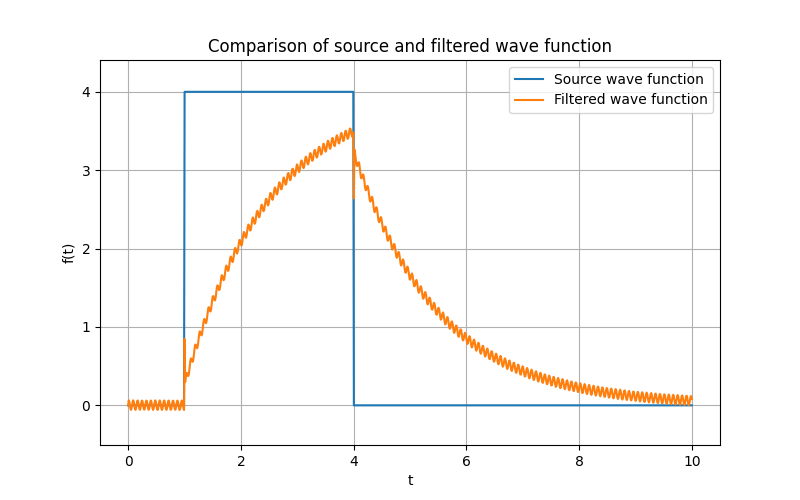
\includegraphics[width=\textwidth]{../results/second/\num/wave_func_cmp.png}
    \caption{Сравнение функции $g(t)$ и $u'(t)$}
    \label{fig:wave_func_cmp_\num}
\end{figure}

Можем сделать вывод, что при увеличении постоянной времени $T$ фильтра, функция становится более гладкой,
при этом меньше похожей на исходную. 

Образ исходной функции и функции после фильтрации приведены на рисунках \ref{fig:wave_func_image_\num}~и~\ref{fig:noised_wave_func_filtered_image_\num}.
Графики модулей соответствующих функций приведены на рисунках~\ref{fig:wave_func_image_abs_\num}~и~\ref{fig:noised_wave_func_filtered_image_abs_\num}, их 
сравнительный график -- на рисунке~\ref{fig:wave_func_image_cmp_\num}.

\begin{figure}[ht!]
    \centering
    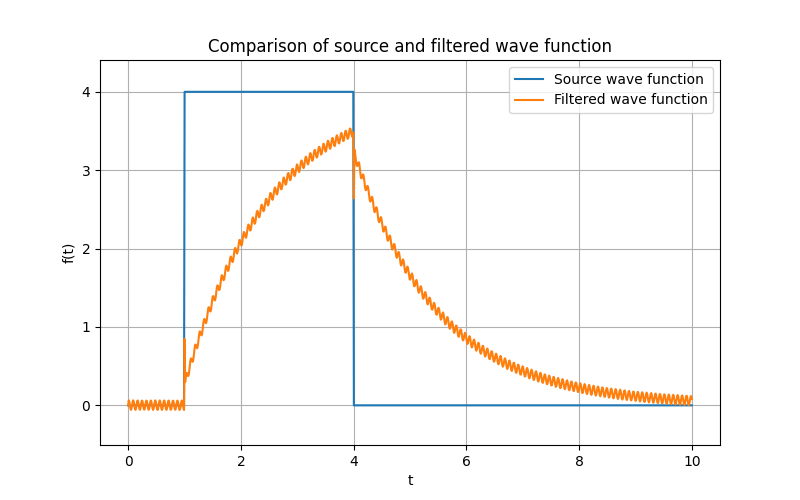
\includegraphics[width=\textwidth]{../results/second/\num/wave_func_cmp.png}
    \caption{Сравнение функции $g(t)$ и $u'(t)$}
    \label{fig:wave_func_cmp_\num}
\end{figure}

\begin{figure}[ht!]
    \centering
    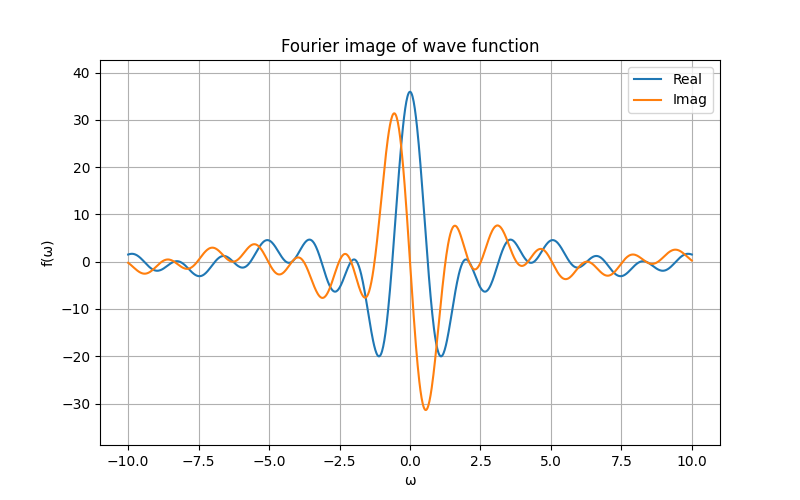
\includegraphics[width=\textwidth]{../results/second/\num/wave_func_image.png}
    \caption{Образ исходной функции $u(t)$.}
    \label{fig:wave_func_image_\num}
\end{figure}

\begin{figure}[ht!]
    \centering
    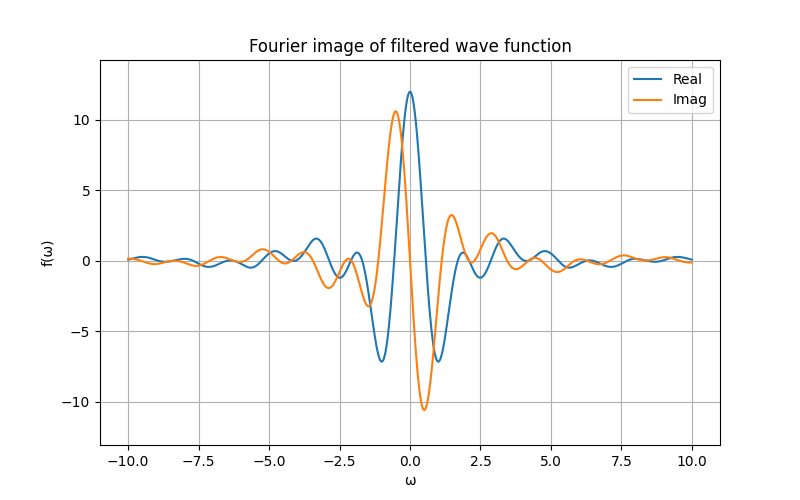
\includegraphics[width=\textwidth]{../results/second/\num/noised_wave_func_filtered_image.png}
    \caption{Образ фильтрованной функции $u'(t)$.}
    \label{fig:noised_wave_func_filtered_image_\num}
\end{figure}

\begin{figure}[ht!]
    \centering
    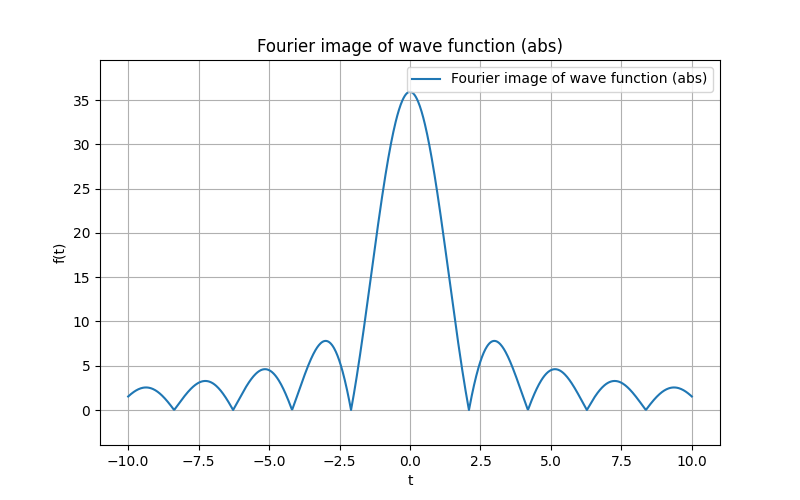
\includegraphics[width=\textwidth]{../results/second/\num/wave_func_image_abs.png}
    \caption{Модуль образа исходной функции $u(t)$.}
    \label{fig:wave_func_image_abs_\num}
\end{figure}

\begin{figure}[ht!]
    \centering
    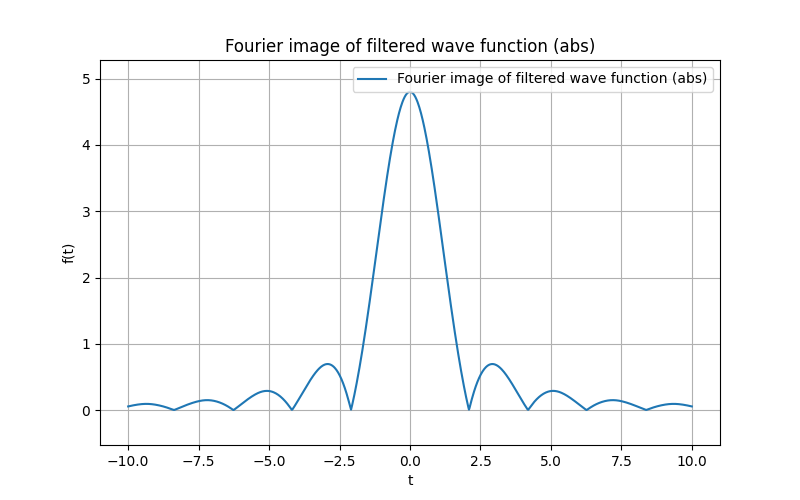
\includegraphics[width=\textwidth]{../results/second/\num/noised_wave_func_filtered_image_abs.png}
    \caption{Модуль образа фильтрованной функции $u'(t)$.}
    \label{fig:noised_wave_func_filtered_image_abs_\num}
\end{figure}

\begin{figure}[ht!]
    \centering
    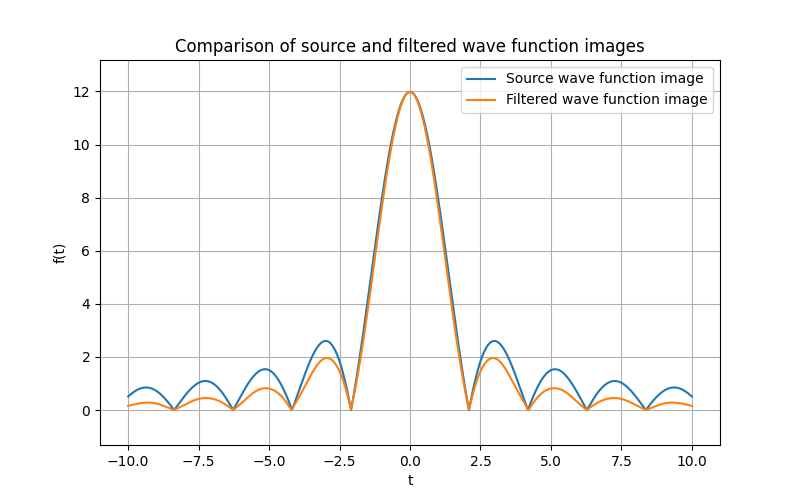
\includegraphics[width=\textwidth]{../results/second/\num/wave_func_image_cmp.png}
    \caption{Сравнение модулей образов исходной и фильтрованной функций.}
    \label{fig:wave_func_image_cmp_\num}
\end{figure}


\FloatBarrier
\subsubsection{Зависимость эффективности фильтрации от параметра a}
\def\T{0.3}
Для исследования данной зависимости рассмотрим функцию $g(t)$ при различных значениях параметра $a$ 
при фильтрации линейным фильтром первого порядка с $T = \T$. 

\def\num{4}
\def\a{10}
Рассмотрим функцию $g(t)$ при параметрах $a=\a$, $t_1 = \from$, $t_2 = \to$ ~(см. рисунок~\ref{fig:wave_func_\num}) 
и ее \textit{зашумленную} версию $u(t)$ с параметрами $b = \b$, $c = \c$, $d = \d$ ~(см. рисунок~\ref{fig:noised_wave_func_\num}).
на промежутке $[0,\L]$. 

\begin{figure}[ht!]
    \centering
    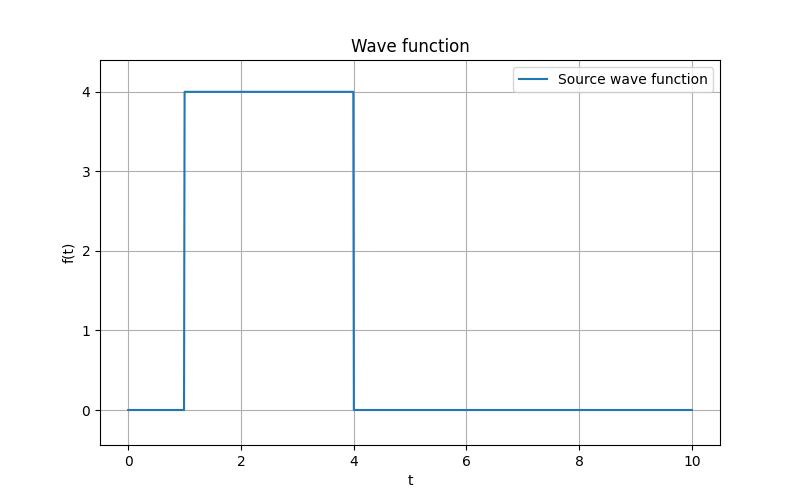
\includegraphics[width=\textwidth]{../results/second/\num/wave_func.png}
    \caption{Функция $g(t)$ с параметрами $a = \a$, $t_1 = \from$, $t_2 = \to$}
    \label{fig:wave_func_\num}
\end{figure}

\begin{figure}[ht!]
    \centering
    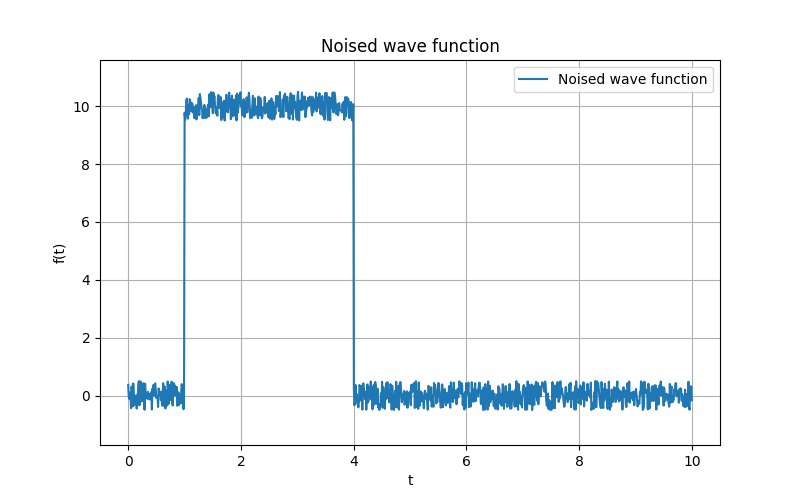
\includegraphics[width=\textwidth]{../results/second/\num/noised_wave_func.png}
    \caption{Функция $u(t)$ с параметрами $b = \b$, $c = \c$, $d = \d$}
    \label{fig:noised_wave_func_\num}
\end{figure}

Результат фильтрации с помощью линейного фильтра первого порядка с $T = \T$ (см. рисунок \ref{fig:noised_wave_func_filtered_\num}).
Сравнительные графики исходной функции и функции после фильтрации представлены на рисунке \ref{fig:wave_func_cmp_\num}.

\begin{figure}[ht!]
    \centering
    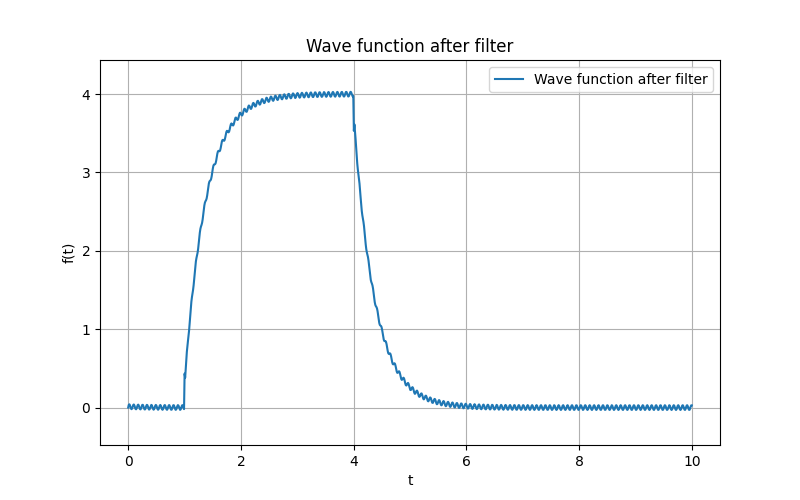
\includegraphics[width=\textwidth]{../results/second/\num/noised_wave_func_filtered.png}
    \caption{Функция $u'(t)$ после применения фильтра}
    \label{fig:noised_wave_func_filtered_\num}
\end{figure}

\begin{figure}[ht!]
    \centering
    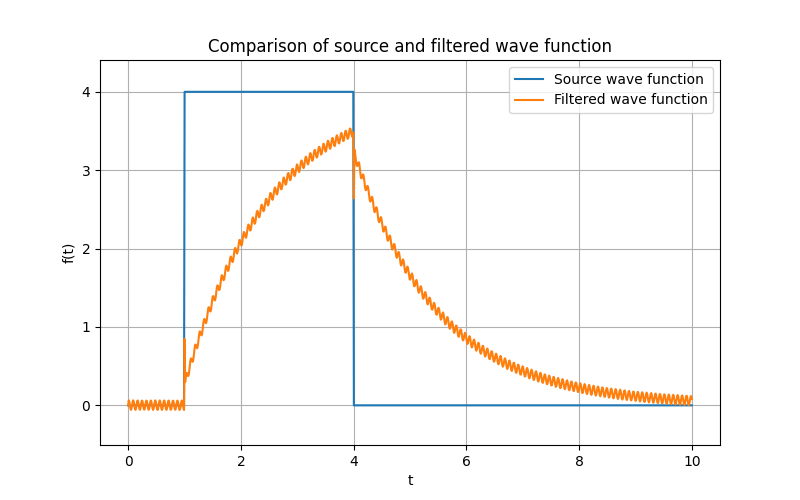
\includegraphics[width=\textwidth]{../results/second/\num/wave_func_cmp.png}
    \caption{Сравнение функции $g(t)$ и $u'(t)$}
    \label{fig:wave_func_cmp_\num}
\end{figure}

Результат практически не отличается от предыдущего случая. Функция стала более гладкой, но при этом
менее похожей на исходную. Фронт и спад так же завалены. 

\def\num{5}
\def\a{30}
Рассмотрим функцию $g(t)$ при параметрах $a=\a$, $t_1 = \from$, $t_2 = \to$ ~(см. рисунок~\ref{fig:wave_func_\num}) 
и ее \textit{зашумленную} версию $u(t)$ с параметрами $b = \b$, $c = \c$, $d = \d$ ~(см. рисунок~\ref{fig:noised_wave_func_\num}).
на промежутке $[0,\L]$. 

\begin{figure}[ht!]
    \centering
    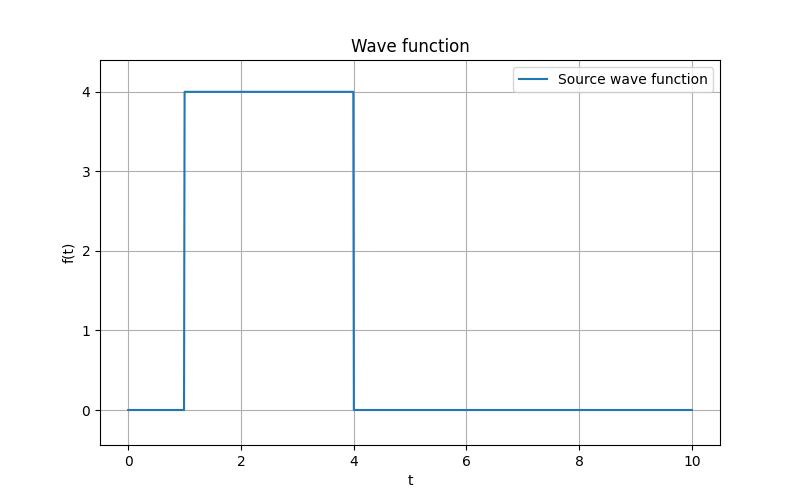
\includegraphics[width=\textwidth]{../results/second/\num/wave_func.png}
    \caption{Функция $g(t)$ с параметрами $a = \a$, $t_1 = \from$, $t_2 = \to$}
    \label{fig:wave_func_\num}
\end{figure}

\begin{figure}[ht!]
    \centering
    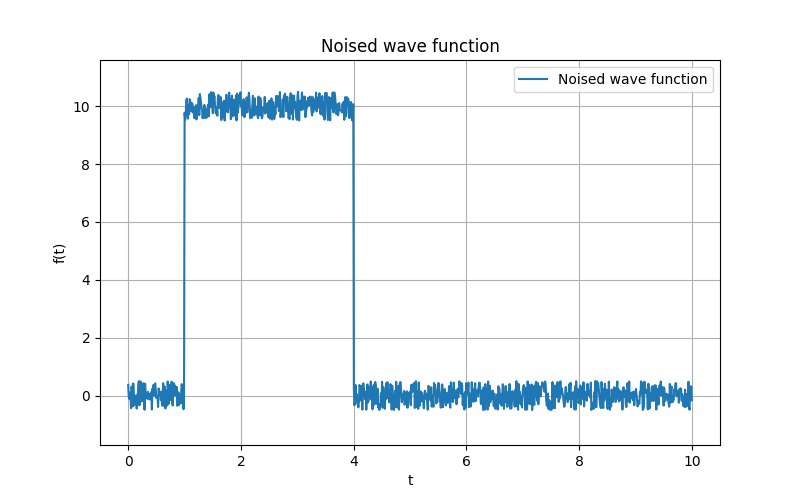
\includegraphics[width=\textwidth]{../results/second/\num/noised_wave_func.png}
    \caption{Функция $u(t)$ с параметрами $b = \b$, $c = \c$, $d = \d$}
    \label{fig:noised_wave_func_\num}
\end{figure}

Результат фильтрации с помощью линейного фильтра первого порядка с $T = \T$ (см. рисунок \ref{fig:noised_wave_func_filtered_\num}).

\begin{figure}[ht!]
    \centering
    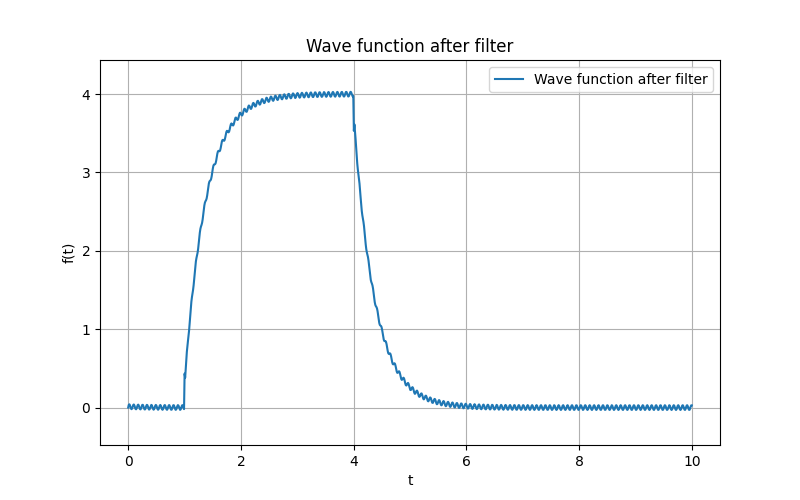
\includegraphics[width=\textwidth]{../results/second/\num/noised_wave_func_filtered.png}
    \caption{Функция $u'(t)$ после применения фильтра}
    \label{fig:noised_wave_func_filtered_\num}
\end{figure}

\begin{figure}[ht!]
    \centering
    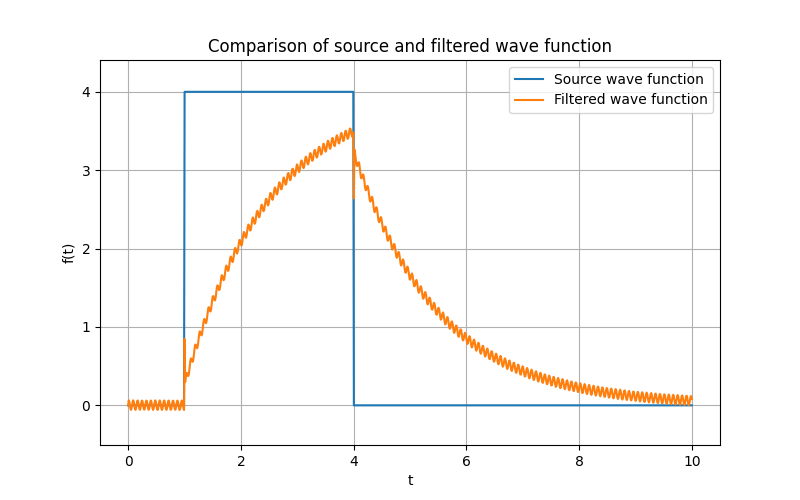
\includegraphics[width=\textwidth]{../results/second/\num/wave_func_cmp.png}
    \caption{Сравнение функции $g(t)$ и $u'(t)$}
    \label{fig:wave_func_cmp_\num}
\end{figure}

Ровно как и в прошлый раз -- никаких изменений. Фронт функции выглядит идентично с поправкой на масштаб.
Сравнительные графики исходной функции и функции после фильтрации представлены на рисунке \ref{fig:wave_func_cmp_\num}.

Можно сделать вывод, что параметр $a$ не влияет на эффективность фильтрации линейным фильтром первого порядка. 
Связано это с тем, что, фильтр первого порядка лишь \textit{масштабирует} функцию согласно его АЧХ. 


\FloatBarrier
\subsection{Специальный фильтр}

Будем рассматривать линейный фильтр второго порядка вида: 
\begin{equation}
    W_2(p) = \frac{(T_1p + 1)^2}{(T_2p + 1)(T_3p + 1)} = \frac{T_1^2p^2 + 2T_1p + 1}{T_2T_3p^2 + (T_2 + T_3)p + 1}
\end{equation}

Для того, чтобы подобрать коэффициенты $T_1$, $T_2$, $T_3$, я рассмотрел данный фильтр в виде произведения двух фильтров первого порядка. 
В ходе рассмотрения графиков АЧХ данных фильтров я пришел к выводу, что, можно ввести параметры $w_0$ и $A$ -- частота, на которой происходить фильтрация и коэффициент подавления на этой частоте соответственно.
коэффициенты исходного фильтра получаются следующим образом:
\begin{equation}
    T_1 = \frac{1}{w_0}, \quad T_2 = \frac{A}{w_0}, \quad T_3 = \frac{1}{Aw_0}
    \label{eq:t_params}
\end{equation}

\def\num{6}
\def\a{4}
\def\from{1}
\def\to{4}
\def\b{0}
\def\c{0.4}
\def\d{80}
\def\L{10}
\def\A{30}
\def\Wz{80}
\def\Tf{\fpeval{round(1 / \Wz, 7)}}
\def\Ts{\fpeval{round(\A / \Wz, 7)}}
\def\Tt{\fpeval{round(1 / (\A * \Wz), 7)}}

\subsubsection{Рассматриваемая функция}
Рассмотрим функцию $g(t)$ при параметрах $a=\a$, $t_1 = \from$, $t_2 = \to$ ~(см. рисунок~\ref{fig:wave_func_\num}) 
и ее \textit{зашумленную} версию $u(t)$ с параметрами $b = \b$, $c = \c$, $d = \d$ ~(см. рисунок~\ref{fig:noised_wave_func_\num}).
на промежутке $[0,\L]$. 

\subsubsection{Графики рассматриваемой и зашумленной функции}
\begin{figure}[ht!]
    \centering
    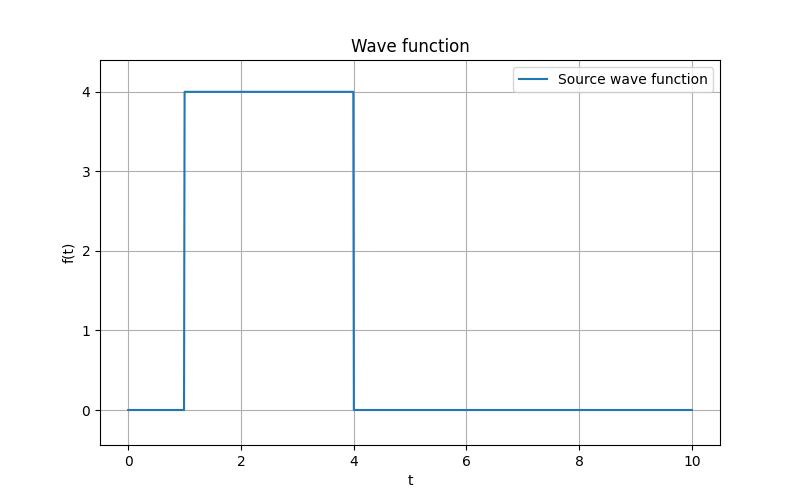
\includegraphics[width=\textwidth]{../results/second/\num/wave_func.png}
    \caption{Функция $g(t)$ с параметрами $a = \a$, $t_1 = \from$, $t_2 = \to$}
    \label{fig:wave_func_\num}
\end{figure}

\begin{figure}[ht!]
    \centering
    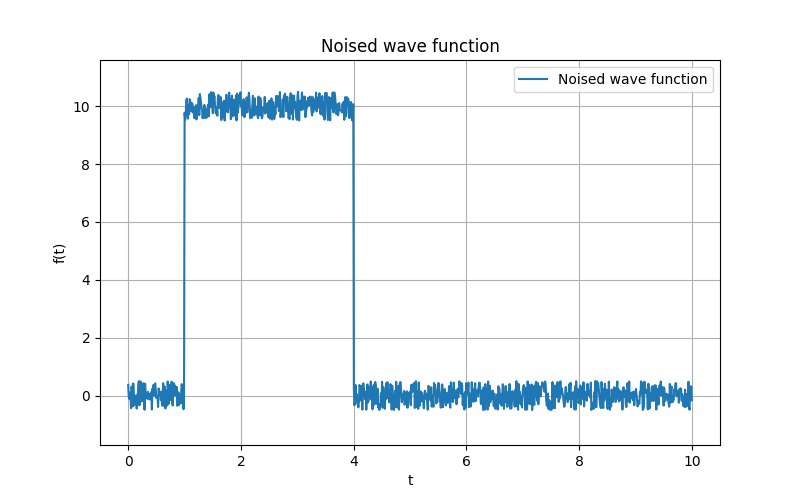
\includegraphics[width=\textwidth]{../results/second/\num/noised_wave_func.png}
    \caption{Функция $u(t)$ с параметрами $b = \b$, $c = \c$, $d = \d$}
    \label{fig:noised_wave_func_\num}
\end{figure}

\FloatBarrier
\subsubsection{Применение фильтра}

Рассмотрим фильтрованную функцию $u'(t)$, которая получается применением линейного фильтра второго порядка с $T_1 = \Tf$, $T_2 = \Ts$, $T_3 = \Tt$ (см. рисунок \ref{fig:noised_wave_func_filtered_\num}).
Значения $T_1,~T_2,~T_3$ получены из формул \eqref{eq:t_params} при $w_0 = \Wz$ и $A = \A$.

\begin{figure}[ht!]
    \centering
    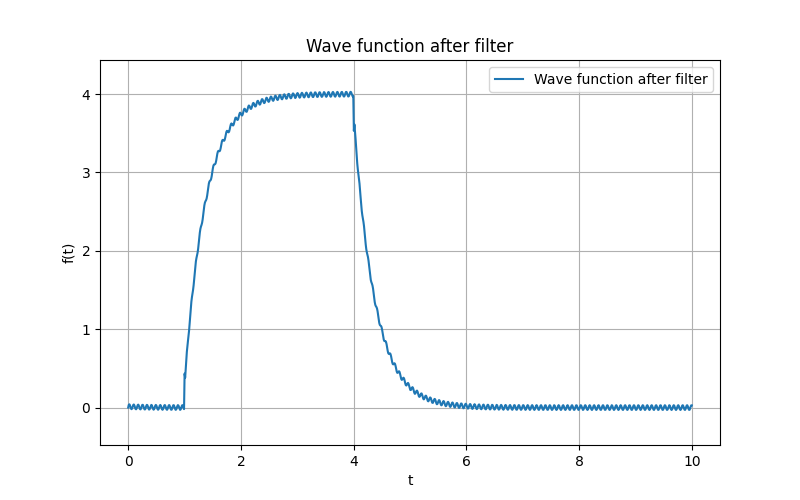
\includegraphics[width=\textwidth]{../results/second/\num/noised_wave_func_filtered.png}
    \caption{Функция $u'(t)$ после применения фильтра}
    \label{fig:noised_wave_func_filtered_\num}
\end{figure}

Видим, что функция после фильтрации стала более гладкой, фронт и спад стали менее выраженными.
Это связано с тем, что фильтр убирает высокочастотные компоненты функции. Убедиться в этом можно 
посмотрев на АЧХ фильтра (см. рисунок \ref{fig:filter_frequency_response_\num} и \ref{fig:filter_frequency_response_log_\num}).

\FloatBarrier
\subsubsection{Амплитудно-частотная характеристика фильтра}
\begin{figure}[ht!]
    \centering
    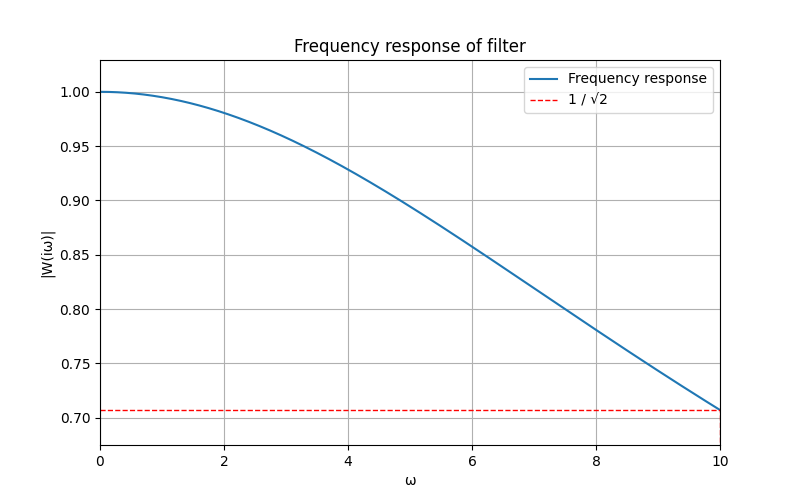
\includegraphics[width=\textwidth]{../results/second/\num/filter_frequency_response.png}
    \caption{АЧХ фильтра второго порядка при $T_1 = \Tf$, $T_2 = \Ts$, $T_3 = \Tt$}
    \label{fig:filter_frequency_response_\num}
\end{figure}

\begin{figure}[ht!]
    \centering
    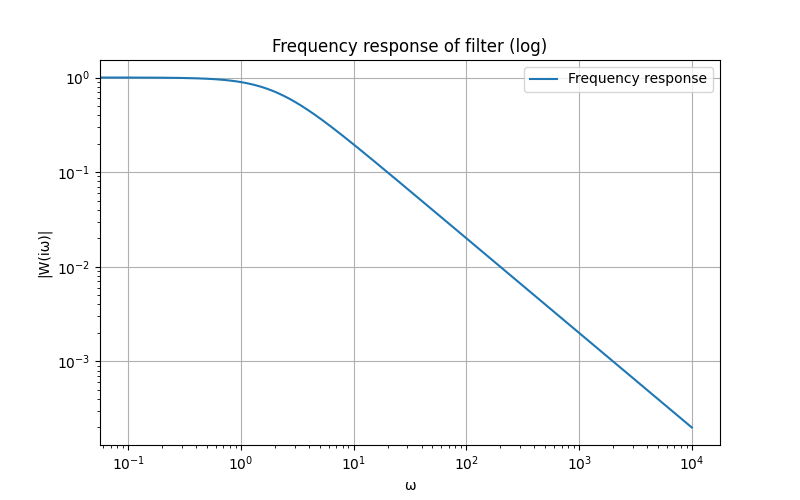
\includegraphics[width=\textwidth]{../results/second/\num/filter_frequency_response_log.png}
    \caption{АЧХ фильтра второго порядка при $T_1 = \Tf$, $T_2 = \Ts$, $T_3 = \Tt$ (логарифмическая шкала)}
    \label{fig:filter_frequency_response_log_\num}
\end{figure}

На логарифмическом графике более заметно, что данный фильтр подавляет частоты в окрестности частоты $w_0 = \Wz$, что и требуется для фильтрации гармонического шума. 
Но, на этом же графике видно, что фильтр, кроме требуемых частот, подавляет довольно большой диапазон частот, что, конечно, сильно сказывается на качестве фильтрации. 
Именно для того, чтобы фильтр минимально срезал нижние частоты, которые необходимы для восстановления исходной функции была выбрана довольно большая частота гармонического шума.

\FloatBarrier
\subsubsection{Результаты фильтрации}
Сравнительный график исходной функции и функции после фильтрации представлен на рисунке \ref{fig:wave_func_cmp_\num}.

\begin{figure}[ht!]
    \centering
    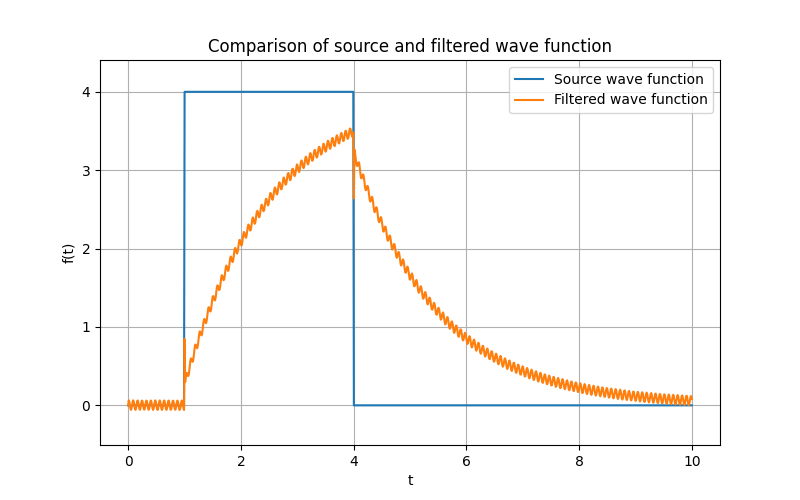
\includegraphics[width=\textwidth]{../results/second/\num/wave_func_cmp.png}
    \caption{Сравнение функции $g(t)$ и $u'(t)$}
    \label{fig:wave_func_cmp_\num}
\end{figure}

Образ исходной функции и функции после фильтрации приведены на рисунках \ref{fig:wave_func_image_\num}~и~\ref{fig:noised_wave_func_filtered_image_\num}.
Графики модулей соответствующих функций приведены на рисунках~\ref{fig:wave_func_image_abs_\num}~и~\ref{fig:noised_wave_func_filtered_image_abs_\num}, их 
сравнительный график -- на рисунке~\ref{fig:wave_func_image_cmp_\num}.

На сравнительном графике (см. рисунок~\ref{fig:wave_func_image_cmp_\num}) видно, что \textit{амплитуда} образа фильтрованного сигнала уменьшается по сравнению 
с образом начальной функции. Результат соответствует АЧХ фильтра (см. рисунок~\ref{fig:filter_frequency_response_\num}).

\begin{figure}[ht!]
    \centering
    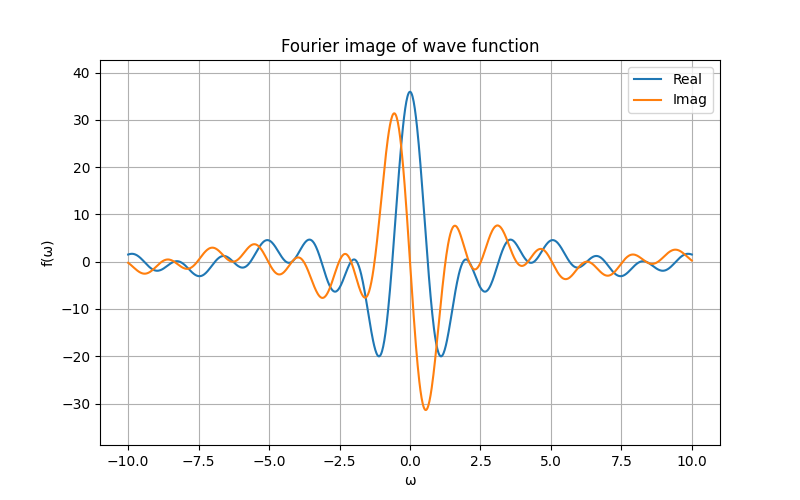
\includegraphics[width=\textwidth]{../results/second/\num/wave_func_image.png}
    \caption{Образ исходной функции $u(t)$.}
    \label{fig:wave_func_image_\num}
\end{figure}

\begin{figure}[ht!]
    \centering
    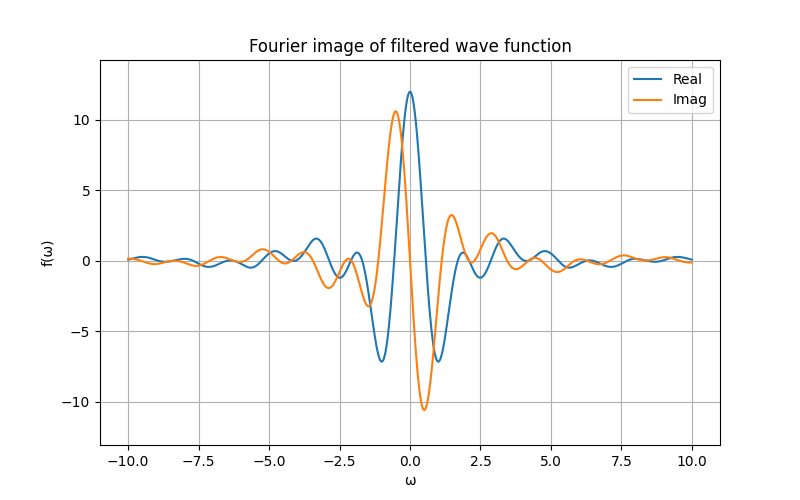
\includegraphics[width=\textwidth]{../results/second/\num/noised_wave_func_filtered_image.png}
    \caption{Образ фильтрованной функции $u'(t)$.}
    \label{fig:noised_wave_func_filtered_image_\num}
\end{figure}

\begin{figure}[ht!]
    \centering
    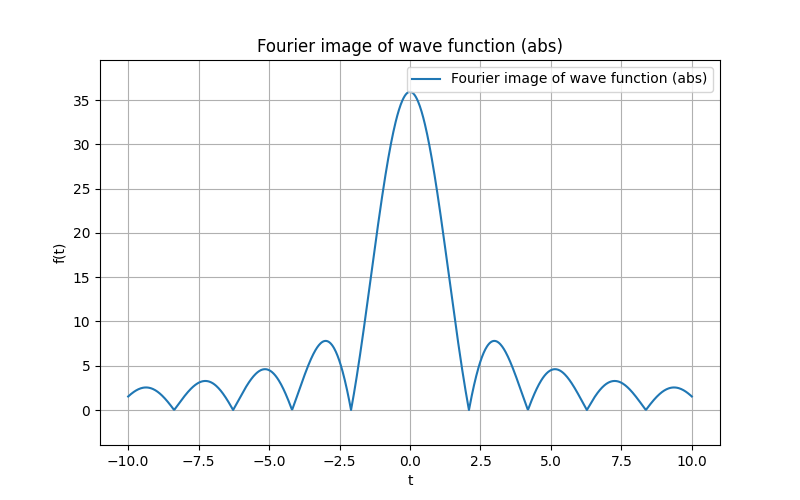
\includegraphics[width=\textwidth]{../results/second/\num/wave_func_image_abs.png}
    \caption{Модуль образа исходной функции $u(t)$.}
    \label{fig:wave_func_image_abs_\num}
\end{figure}

\begin{figure}[ht!]
    \centering
    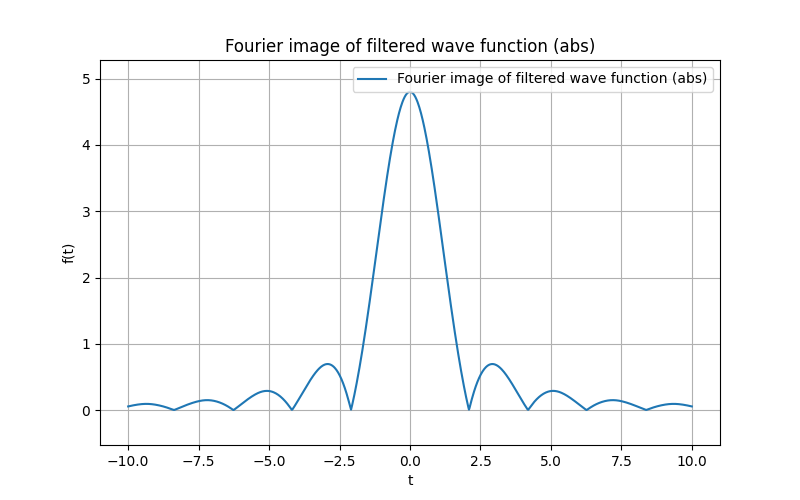
\includegraphics[width=\textwidth]{../results/second/\num/noised_wave_func_filtered_image_abs.png}
    \caption{Модуль образа фильтрованной функции $u'(t)$.}
    \label{fig:noised_wave_func_filtered_image_abs_\num}
\end{figure}

\begin{figure}[ht!]
    \centering
    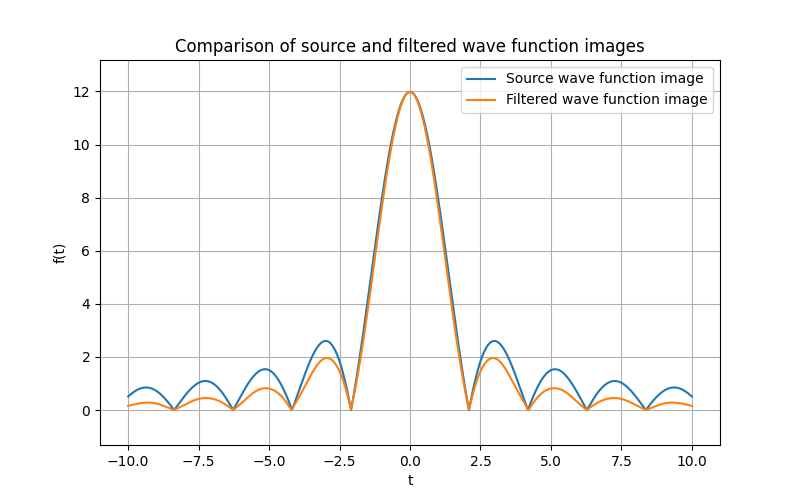
\includegraphics[width=\textwidth]{../results/second/\num/wave_func_image_cmp.png}
    \caption{Сравнение модулей образов исходной и фильтрованной функций.}
    \label{fig:wave_func_image_cmp_\num}
\end{figure}

\FloatBarrier
\subsubsection{Фильтрация шума меньшей частоты}

\def\num{7}
\def\a{4}
\def\from{1}
\def\to{4}
\def\b{0}
\def\c{0.4}
\def\d{20}
\def\L{10}
\def\A{30}
\def\Wz{20}
\def\Tf{\fpeval{round(1 / \Wz, 7)}}
\def\Ts{\fpeval{round(\A / \Wz, 7)}}
\def\Tt{\fpeval{round(1 / (\A * \Wz), 7)}}

Теперь рассмотрим функцию с гармоническом шумом меньшей частоты, чем в предыдущем случае: 
$g(t)$ при параметрах $a=\a$, $t_1 = \from$, $t_2 = \to$ ~(см. рисунок~\ref{fig:wave_func_\num}) 
и ее \textit{зашумленную} версию $u(t)$ с параметрами $b = \b$, $c = \c$, $d = \d$ ~(см. рисунок~\ref{fig:noised_wave_func_\num}).
на промежутке $[0,\L]$. 

\begin{figure}[ht!]
    \centering
    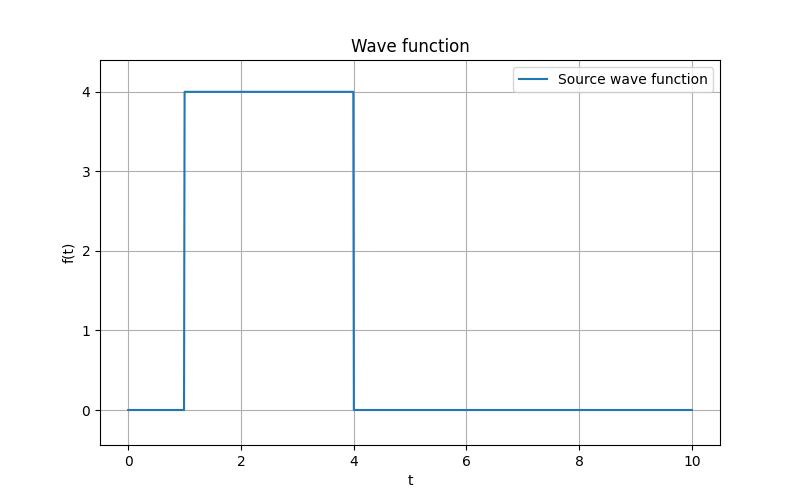
\includegraphics[width=\textwidth]{../results/second/\num/wave_func.png}
    \caption{Функция $g(t)$ с параметрами $a = \a$, $t_1 = \from$, $t_2 = \to$}
    \label{fig:wave_func_\num}
\end{figure}

\begin{figure}[ht!]
    \centering
    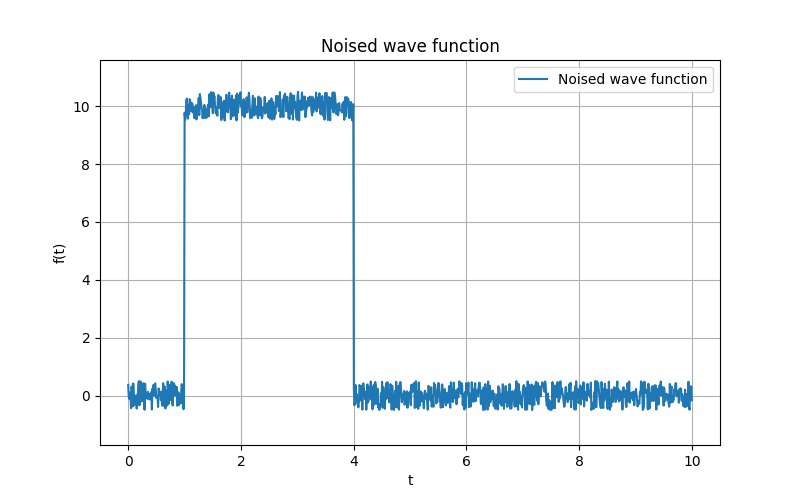
\includegraphics[width=\textwidth]{../results/second/\num/noised_wave_func.png}
    \caption{Функция $u(t)$ с параметрами $b = \b$, $c = \c$, $d = \d$}
    \label{fig:noised_wave_func_\num}
\end{figure}

Рассмотрим фильтрованную функцию $u'(t)$, которая получается применением линейного фильтра второго порядка с $T_1 = \Tf$, $T_2 = \Ts$, $T_3 = \Tt$ (см. рисунок \ref{fig:noised_wave_func_filtered_\num}).
Значения $T_1,~T_2,~T_3$ получены из формул \eqref{eq:t_params} при $w_0 = \Wz$ и $A = \A$.

\begin{figure}[ht!]
    \centering
    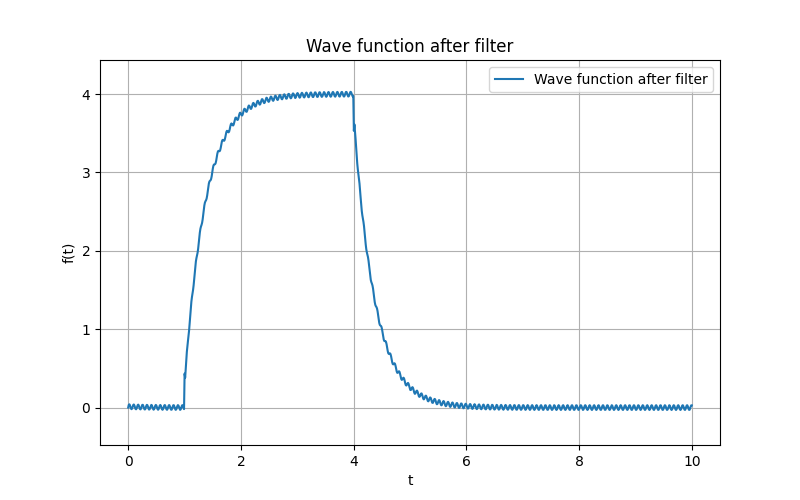
\includegraphics[width=\textwidth]{../results/second/\num/noised_wave_func_filtered.png}
    \caption{Функция $u'(t)$ после применения фильтра}
    \label{fig:noised_wave_func_filtered_\num}
\end{figure}

На рисунке~\ref{fig:noised_wave_func_filtered_\num} видно, что гармонический шум действительно уменьшился, при этом,
фронт и спад функции стали менее выраженными. Это связано с тем, что фильтр убирает не только частоты гармонического шума,
но и некоторый диапазон частот рядом с ним, что и приводит к сглаживанию функции.
Убедить в этом можно посмотрев на графики АЧХ данного фильтра (см. рисунок \ref{fig:filter_frequency_response_\num} и \ref{fig:filter_frequency_response_log_\num}).

\begin{figure}[ht!]
    \centering
    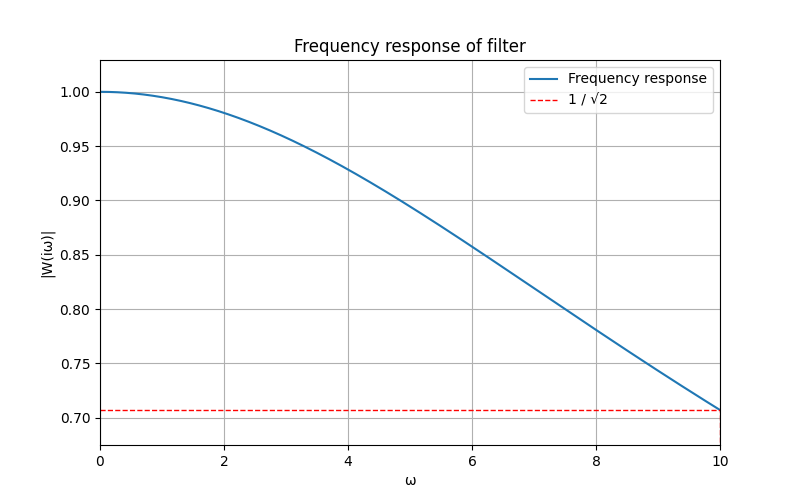
\includegraphics[width=\textwidth]{../results/second/\num/filter_frequency_response.png}
    \caption{АЧХ фильтра второго порядка при $T_1 = \Tf$, $T_2 = \Ts$, $T_3 = \Tt$}
    \label{fig:filter_frequency_response_\num}
\end{figure}

\begin{figure}[ht!]
    \centering
    \includegraphics[width=\textwidth]{../results/second/\num/filter_frequency_response_log.png}
    \caption{АЧХ фильтра второго порядка при $T_1 = \Tf$, $T_2 = \Ts$, $T_3 = \Tt$ (логарифмическая шкала)}
    \label{fig:filter_frequency_response_log_\num}
\end{figure}

Сравнительный график исходной и фильтрованной функции приведен на рисунке~\ref{fig:wave_func_cmp_\num}.
\begin{figure}[ht!]
    \centering
    \includegraphics[width=\textwidth]{../results/second/\num/wave_func_cmp.png}
    \caption{Сравнение функции $g(t)$ и $u'(t)$}
    \label{fig:wave_func_cmp_\num}
\end{figure}

\FloatBarrier
\subsubsection{Фильтрация шума большей частоты}

\def\num{8}
\def\a{4}
\def\from{1}
\def\to{4}
\def\b{0}
\def\c{1}
\def\d{2000}
\def\L{10}
\def\A{300}
\def\Wz{2000}
\def\Tf{\fpeval{round(1 / \Wz, 7)}}
\def\Ts{\fpeval{round(\A / \Wz, 7)}}
\def\Tt{\fpeval{round(1 / (\A * \Wz), 7)}}

Теперь рассмотрим более удачный случай, когда гармонический шум имеет большую частоту. Такую, что
при применении фильтра не будет захватываться диапазон частот, необходимый для восстановления исходной функции.

Рассмотрим функцию $g(t)$ при параметрах $a=\a$, $t_1 = \from$, $t_2 = \to$ ~(см. рисунок~\ref{fig:wave_func_\num}) 
и ее \textit{зашумленную} версию $u(t)$ с параметрами $b = \b$, $c = \c$, $d = \d$ ~(см. рисунок~\ref{fig:noised_wave_func_\num}).
на промежутке $[0,\L]$. 

\begin{figure}[ht!]
    \centering
    \includegraphics[width=\textwidth]{../results/second/\num/wave_func.png}
    \caption{Функция $g(t)$ с параметрами $a = \a$, $t_1 = \from$, $t_2 = \to$}
    \label{fig:wave_func_\num}
\end{figure}

\begin{figure}[ht!]
    \centering
    \includegraphics[width=\textwidth]{../results/second/\num/noised_wave_func.png}
    \caption{Функция $u(t)$ с параметрами $b = \b$, $c = \c$, $d = \d$}
    \label{fig:noised_wave_func_\num}
\end{figure}

Рассмотрим фильтрованную функцию $u'(t)$, которая получается применением линейного фильтра второго порядка с $T_1 = \Tf$, $T_2 = \Ts$, $T_3 = \Tt$ (см. рисунок \ref{fig:noised_wave_func_filtered_\num}).
Значения $T_1,~T_2,~T_3$ получены из формул \eqref{eq:t_params} при $w_0 = \Wz$ и $A = \A$.
АЧХ данного фильтра приведена на рисунках \ref{fig:filter_frequency_response_\num} и \ref{fig:filter_frequency_response_log_\num}.

\begin{figure}[ht!]
    \centering
    \includegraphics[width=\textwidth]{../results/second/\num/noised_wave_func_filtered.png}
    \caption{Функция $u'(t)$ после применения фильтра}
    \label{fig:noised_wave_func_filtered_\num}
\end{figure}

\begin{figure}[ht!]
    \centering
    \includegraphics[width=\textwidth]{../results/second/\num/filter_frequency_response.png}
    \caption{АЧХ фильтра второго порядка при $T_1 = \Tf$, $T_2 = \Ts$, $T_3 = \Tt$}
    \label{fig:filter_frequency_response_\num}
\end{figure}

\begin{figure}[ht!]
    \centering
    \includegraphics[width=\textwidth]{../results/second/\num/filter_frequency_response_log.png}
    \caption{АЧХ фильтра второго порядка при $T_1 = \Tf$, $T_2 = \Ts$, $T_3 = \Tt$ (логарифмическая шкала)}
    \label{fig:filter_frequency_response_log_\num}
\end{figure}

Видно, что гармонический шум практически полностью был убран, при этом сама функция сохранила свой вид. 
Сравнительные графики исходной и фильтрованной функции приведены на рисунке~\ref{fig:wave_func_cmp_\num}.

\begin{figure}[ht!]
    \centering
    \includegraphics[width=\textwidth]{../results/second/\num/wave_func_cmp.png}
    \caption{Сравнение функции $g(t)$ и $u'(t)$}
    \label{fig:wave_func_cmp_\num}
\end{figure}

\subsubsection{Исследование влияния параметра c на результат фильтрации}


\def\num{8}
\def\a{4}
\def\from{1}
\def\to{4}
\def\b{0}
\def\c{2}
\def\d{80}
\def\L{10}
\def\A{30}
\def\Wz{80}
\def\Tf{\fpeval{round(1 / \Wz, 7)}}
\def\Ts{\fpeval{round(\A / \Wz, 7)}}
\def\Tt{\fpeval{round(1 / (\A * \Wz), 7)}}

Рассмотрим функцию $g(t)$ при параметрах $a=\a$, $t_1 = \from$, $t_2 = \to$ ~(см. рисунок~\ref{fig:wave_func_\num}) 
и ее \textit{зашумленную} версию $u(t)$ с параметрами $b = \b$, $c = \c$, $d = \d$ ~(см. рисунок~\ref{fig:noised_wave_func_\num}).
на промежутке $[0,\L]$. 

\begin{figure}[ht!]
    \centering
    \includegraphics[width=\textwidth]{../results/second/\num/wave_func.png}
    \caption{Функция $g(t)$ с параметрами $a = \a$, $t_1 = \from$, $t_2 = \to$}
    \label{fig:wave_func_\num}
\end{figure}

\begin{figure}[ht!]
    \centering
    \includegraphics[width=\textwidth]{../results/second/\num/noised_wave_func.png}
    \caption{Функция $u(t)$ с параметрами $b = \b$, $c = \c$, $d = \d$}
    \label{fig:noised_wave_func_\num}
\end{figure}

Рассмотрим фильтрованную функцию $u'(t)$, которая получается применением линейного фильтра второго порядка с $T_1 = \Tf$, $T_2 = \Ts$, $T_3 = \Tt$ (см. рисунок \ref{fig:noised_wave_func_filtered_\num}).
Значения $T_1,~T_2,~T_3$ получены из формул \eqref{eq:t_params} при $w_0 = \Wz$ и $A = \A$.

\begin{figure}[ht!]
    \centering
    \includegraphics[width=\textwidth]{../results/second/\num/noised_wave_func_filtered.png}
    \caption{Функция $u'(t)$ после применения фильтра}
    \label{fig:noised_wave_func_filtered_\num}
\end{figure}

Сравнительный график исходной функции и функции после фильтрации представлен на рисунке \ref{fig:wave_func_cmp_\num}.

\begin{figure}[ht!]
    \centering
    \includegraphics[width=\textwidth]{../results/second/\num/wave_func_cmp.png}
    \caption{Сравнение функции $g(t)$ и $u'(t)$}
    \label{fig:wave_func_cmp_\num}
\end{figure}

Видно, что, как и в первом случае, гармонический шум был успешно убран, несмотря на то, 
что его амплитуда довольно сильно увеличилась (более, чем в 4 раза). Это связано с тем, что 
фильтр подавляет частоты, на которых находится гармонический шум, при этом шум любой амплитуды
будет подавляться пропорционально. 

